\documentclass[aspectratio=169]{../latex_main/tntbeamer}  % you can pass all options of the beamer class, e.g., 'handout' or 'aspectratio=43'
\usepackage{dsfont}
\usepackage{bm}
\usepackage[english]{babel}
\usepackage[T1]{fontenc}
%\usepackage[utf8]{inputenc}
\usepackage{graphicx}
\graphicspath{ {./figures/} }
\usepackage{algorithm}
\usepackage[ruled,vlined,algo2e,linesnumbered]{algorithm2e}
\usepackage{hyperref}
\usepackage{booktabs}
\usepackage{mathtools}

\usepackage{amsmath,amssymb}

\DeclareMathOperator*{\argmax}{arg\,max}
\DeclareMathOperator*{\argmin}{arg\,min}

\usepackage{amsbsy}
\newcommand{\vect}[1]{\bm{#1}}
%\newcommand{\vect}[1]{\boldsymbol{#1}}

\usepackage{pgfplots}
\pgfplotsset{compat=1.16}
\usepackage{tikz}
\usetikzlibrary{trees} 
\usetikzlibrary{shapes.geometric}
\usetikzlibrary{positioning,shapes,shadows,arrows,calc,mindmap}
\usetikzlibrary{positioning,fadings,through}
\usetikzlibrary{decorations.pathreplacing}
\usetikzlibrary{intersections}
\pgfdeclarelayer{background}
\pgfdeclarelayer{foreground}
\pgfsetlayers{background,main,foreground}
\tikzstyle{activity}=[rectangle, draw=black, rounded corners, text centered, text width=8em]
\tikzstyle{data}=[rectangle, draw=black, text centered, text width=8em]
\tikzstyle{myarrow}=[->, thick, draw=black]

% Define the layers to draw the diagram
\pgfdeclarelayer{background}
\pgfdeclarelayer{foreground}
\pgfsetlayers{background,main,foreground}

% Requires XeLaTeX or LuaLaTeX
%\usepackage{unicode-math}

\usepackage{fontspec}
%\setsansfont{Arial}
\setsansfont{RotisSansSerifStd}[ 
Path=../latex_main/fonts/,
Extension = .otf,
UprightFont = *-Regular,  % or *-Light
BoldFont = *-ExtraBold,  % or *-Bold
ItalicFont = *-Italic
]
\setmonofont{Cascadia Mono}[
Scale=0.8
]

% scale factor adapted; mathrm font added (Benjamin Spitschan @TNT, 2021-06-01)
%\setmathfont[Scale=1.05]{Libertinus Math}
%\setmathrm[Scale=1.05]{Libertinus Math}

% other available math fonts are (not exhaustive)
% Latin Modern Math
% XITS Math
% Libertinus Math
% Asana Math
% Fira Math
% TeX Gyre Pagella Math
% TeX Gyre Bonum Math
% TeX Gyre Schola Math
% TeX Gyre Termes Math

% Literature References
\newcommand{\lit}[2]{\href{#2}{\footnotesize\color{black!60}[#1]}}

%%% Beamer Customization
%----------------------------------------------------------------------
% (Don't) Show sections in frame header. Options: 'sections', 'sections light', empty
\setbeamertemplate{headline}{empty}

% Add header logo for normal frames
\setheaderimage{
	% 
\includegraphics[height=\logoheight]{figures/TNT_darkv4.pdf}
	
\includegraphics[height=\logoheight]{../latex_main/figures/luh_logo_rgb_0_80_155.pdf}
	% 
\includegraphics[height=\logoheight]{figures/logo_tntluh.pdf}
}

% Header logo for title page
\settitleheaderimage{
	% 
\includegraphics[height=\logoheight]{figures/TNT_darkv4.pdf}
	
\includegraphics[height=\logoheight]{../latex_main/figures/luh_logo_rgb_0_80_155.pdf}
	% 
\includegraphics[height=\logoheight]{figures/logo_tntluh.pdf}
}

% Title page: tntdefault 
\setbeamertemplate{title page}[tntdefault]  % or luhstyle
% Add optional title image here
%\addtitlepageimagedefault{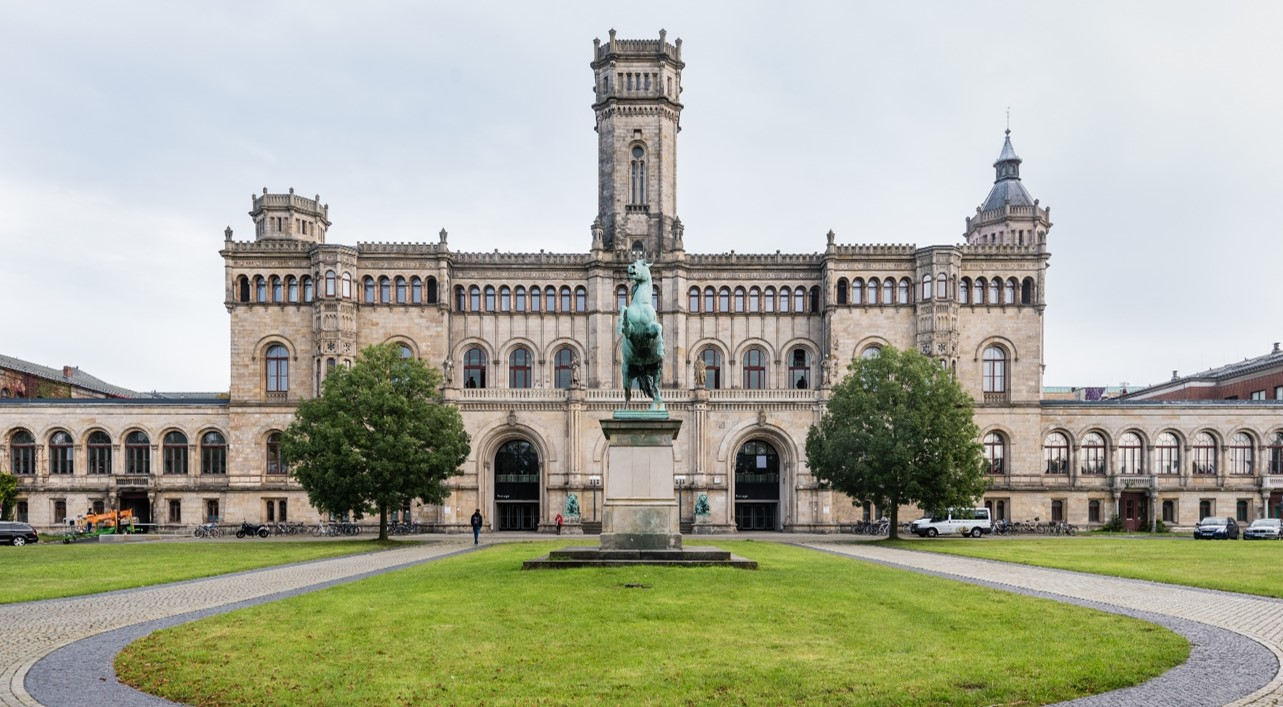
\includegraphics[width=0.65\textwidth]{figures/luh_default_presentation_title_image.jpg}}

% Title page: luhstyle
% \setbeamertemplate{title page}[luhstyle]
% % Add optional title image here
% \addtitlepageimage{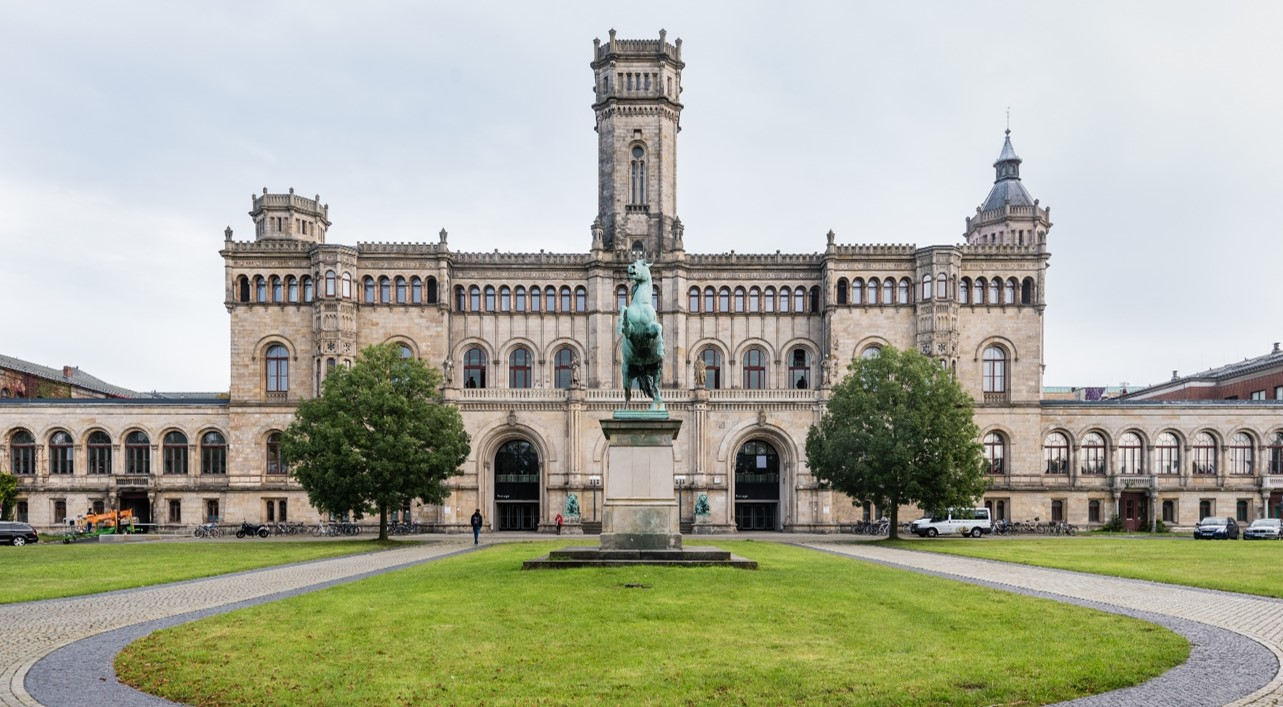
\includegraphics[width=0.75\textwidth]{figures/luh_default_presentation_title_image.jpg}}

\author[Abedjan \& Lindauer]{Ziawasch Abedjan \& Marius Lindauer\\[1em]
	
\includegraphics[height=\logoheight]{../latex_main/figures/luh_logo_rgb_0_80_155.pdf}\qquad
	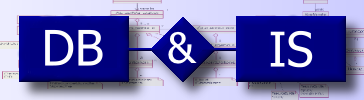
\includegraphics[height=\logoheight]{../latex_main/figures/DBIS_Kurzlogo.png}\qquad

\includegraphics[height=\logoheight]{../latex_main/figures/TNT_darkv4}\qquad

\includegraphics[height=\logoheight]{../latex_main/figures/L3S.jpg}	}
\date{Summer Term 2022; \hspace{0.5em} {
\includegraphics[height=1.5em]{../latex_main/figures/Cc-by-nc-sa_icon.svg.png}}; based on \href{https://ds100.org/fa21/}{[DS100]}
}


%%% Custom Packages
%----------------------------------------------------------------------
% Create dummy content
\usepackage{blindtext}

% Adds a frame with the current page layout. Just call \layout inside of a frame.
\usepackage{layout}


%%% Macros
%\renewcommand{\vec}[1]{\mathbf{#1}}
% \usepackage{bm}
%\let\vecb\bm

\title[Introduction]{DS: Clustering, Part 1}
\subtitle{Overview}

\graphicspath{ {./figure/} }
%\institute{}


\begin{document}
	
	\maketitle
	\begin{frame}{Overview}
	    We’ve completed the core narrative arc of our class
	    \begin{itemize}
	        \item Sampling
	        \item Problem: Tabular Data Manipulation
	        \begin{itemize}
	            \item Solutions: Pandas and SQL
	        \end{itemize}
	        \item Problem: Regression and Classification
	        \begin{itemize}
	            \item Solution: Linear Models and Decision Trees
	        \end{itemize}
	        \item Problem: Dimensionality Reduction
	        \begin{itemize}
	            \item Solution: PCA
	        \end{itemize}
	    \end{itemize}
	    It turns out that these last two problems are examples of Machine Learning algorithms that “learn” from data
	\end{frame}
	
	
	\begin{frame}{Review: Taxonomy of Machine Learning}
	    \begin{figure}
	        \centering
	        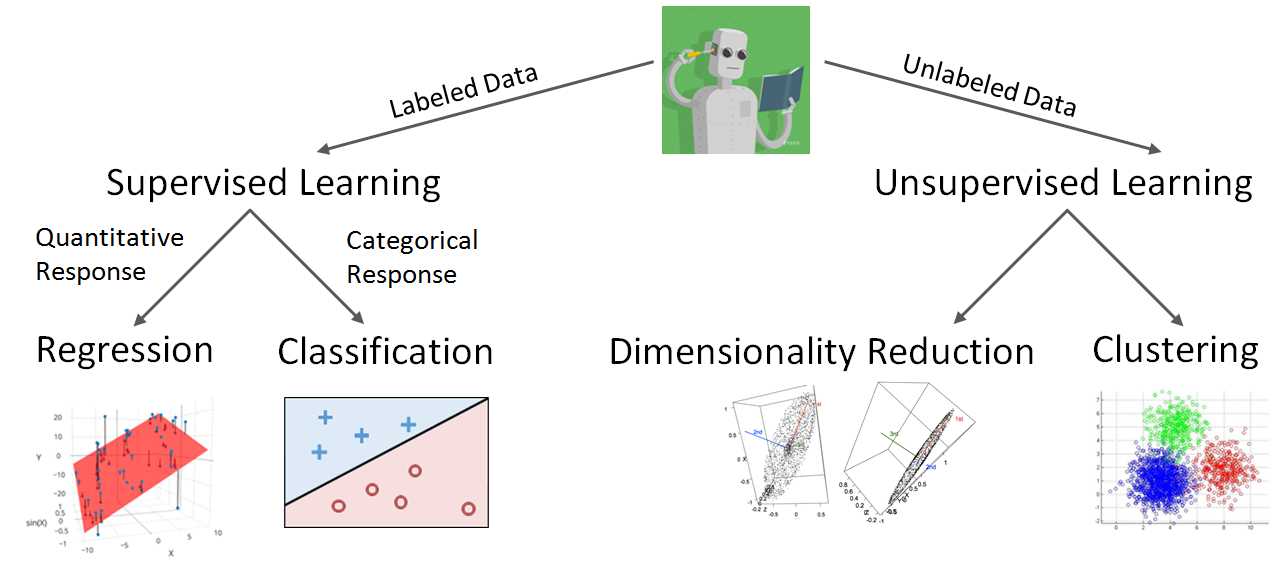
\includegraphics[scale=.4]{Bild1}
	    \end{figure}
	\end{frame}
	
	
	\begin{frame}{Review: Taxonomy of Machine Learning}
	    \begin{columns}
	        \begin{column}{.5\textwidth}
	                \begin{figure}
	                    \centering
	                    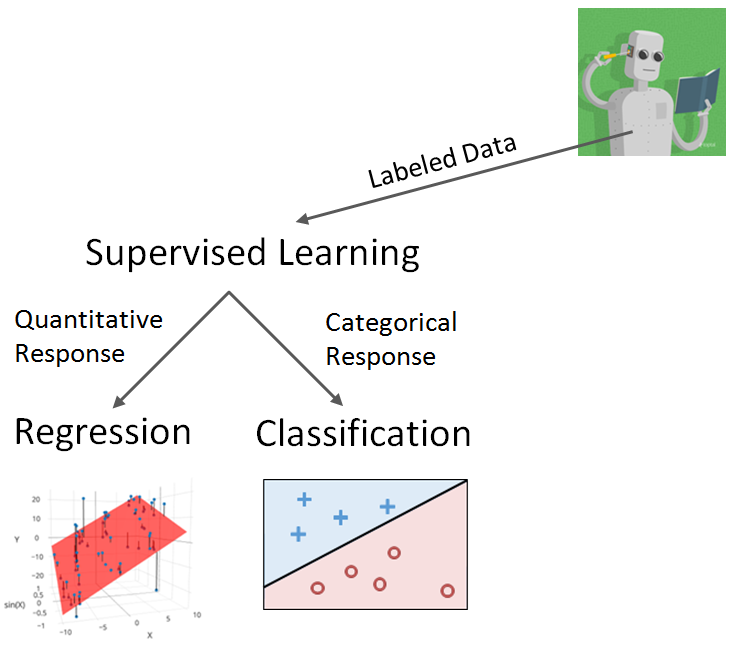
\includegraphics[scale=.33]{Bild2}
	                \end{figure}
	        \end{column}
	        
	        
	        \begin{column}{.5\textwidth}
	            \\
	            \bigskip In “Supervised Learning”:
	                \begin{itemize}
	                    \item Goal is to create a function that maps inputs to outputs
	                    \item Model is learned from example input/output pairs. Each pair consists of:
	                    \begin{itemize}
	                        \item Input vector
	                        \item Output value (label)
	                    \end{itemize}
	                    \item Regression: Output value is quantitative
	                    \item Classification: Output value is categorical
	                \end{itemize}
	        \end{column}
	    \end{columns}
	\end{frame}
	
	
	
	\begin{frame}{Review: Taxonomy of Machine Learning}
	    \begin{columns}
	    

	        \begin{column}{.5\textwidth}
	               In “Unsupervised Learning”:
	               \begin{itemize}
	                   \item Goal is to identify patterns in unlabeled data
	                   \begin{itemize}
	                       \item We do not have input/output pairs
	                   \end{itemize}
	               \end{itemize}
	               Note that if even if we have labels, we can still use clustering to “figure out” the labels
	        \end{column}
	        
	        
	        \begin{column}{.5\textwidth}
	                 \begin{figure}
	                    \centering
	                    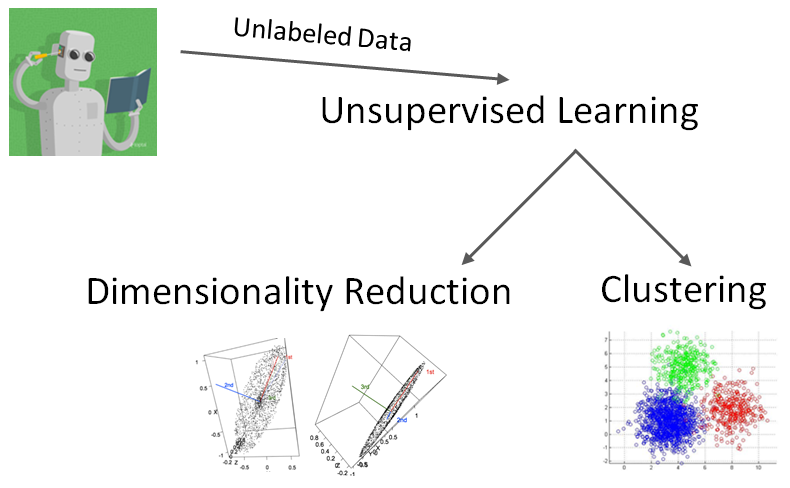
\includegraphics[scale=.33]{Bild3}
	                \end{figure}
	        \end{column}
	    \end{columns}
	\end{frame}
	
	
	
	\begin{frame}{Clustering Example}
	    \begin{columns}
	    

	        \begin{column}{.5\textwidth}
	               Consider the figure shown from Fall 2019 Midterm 2
	               \begin{itemize}
	                   \item Recall that each point represents the 1st and 2nd PC of how much time patrons spent at 8 different zoo exhibits
	               \end{itemize}
	                   Goal of clustering: Assign each point to a cluster\\
	                   \bigskip
	                   Goal of clustering: Assign each point to a cluster
	                   \begin{itemize}
	                       \item We don’t have labels for each visitor
	                       \item Want to infer pattern even without labels
	                   \end{itemize}


	        \end{column}
	        
	        
	        \begin{column}{.5\textwidth}
	                 \begin{figure}
	                    \centering
	                    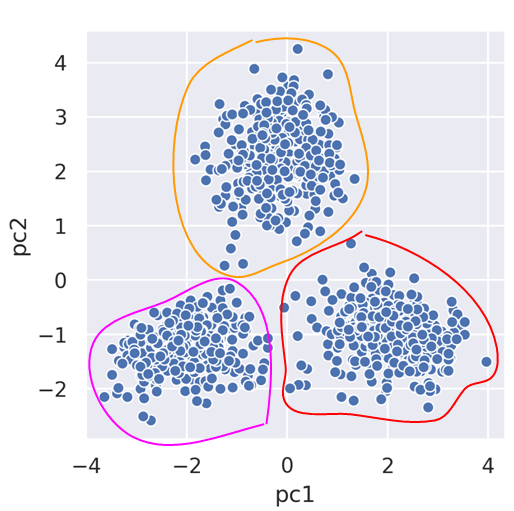
\includegraphics[scale=.4]{Bild4}
	                \end{figure}
	        \end{column}
	    \end{columns}
	\end{frame}
	
	
	
	\begin{frame}{Clustering Example 1: Netflix}
	    Suppose you’re Netflix and have information on customer viewing habits
	    \begin{itemize}
	        \item Can use clustering to assign each person or show to a “cluster”
	        \item Don’t have to define clusters in advance
	    \end{itemize}
	    \bigskip
	    Clustering is different from classification
	    \begin{itemize}
	        \item With classification, you have to decide on labels in advance
	        \item Clustering discovers groups automatically
	    \end{itemize}
	\end{frame}
	
	
	\begin{frame}{Clustering Example 1: Netflix}
	    \begin{figure}
	        \centering
	        
\includegraphics[scale=.4]{Bild5}
	    \end{figure}
	\end{frame}
	
	
	
	\begin{frame}{Clustering Example 2: Clustering Students}
	    In 2018, as a tiny part of a project working to understand factors that affect 61B student success, Prof. Josh Hug tried clustering students based on:
	    \begin{itemize}
	        \item Time and number of posts on Piazza
	        \item Time and number of submissions to Gradescope
	        \item Time and number of submissions to GitHub (basically whenever students saved work)
	    \end{itemize}
	    \bigskip
	    Clustering algorithm automatically identified procrastinating students
	    \bigskip
	    This result wasn’t particularly useful, but it was somewhat interesting

	\end{frame}
	
	
	
	\begin{frame}{Clustering Example 3: Reverse Engineering Biology}
	    \begin{columns}
	    

	        \begin{column}{.5\textwidth}
	               In plot to the right:
	               \begin{itemize}
	                   \item Rows are conditions (e.g. a row might be: “poured acid on the cells”)
	                   \item Columns are genes
	               \end{itemize}
	                   
	                   \bigskip
	                   Green indicates that the gene was ~off
	                   \begin{itemize}
	                       \item The ~9 genes on the left all got turned off by the 6 experiments at the top
	                   \end{itemize}
	                   
	                   \bigskip
                        Clustering brings similar observations together

	        \end{column}
	        
	        
	        \begin{column}{.5\textwidth}
	                 \begin{figure}
	                    \centering
	                    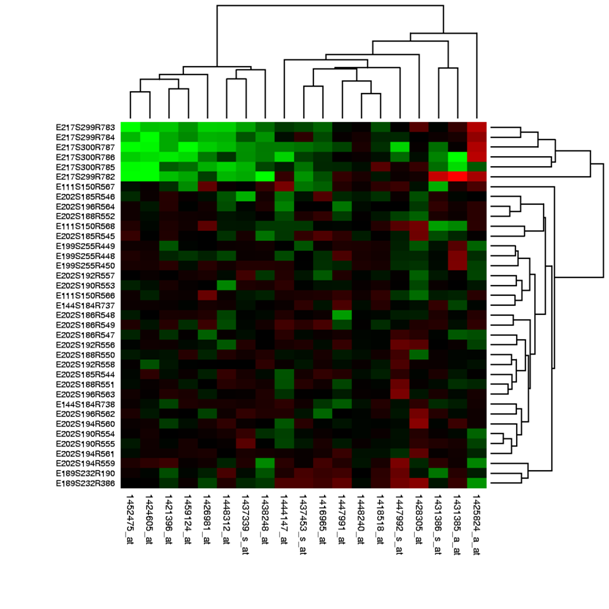
\includegraphics[scale=.6]{Bild6}
	                \end{figure}
	        \end{column}
	    \end{columns}
	\end{frame}
\end{document}